\chapter{Analyse du besoin}

\section{Diagramme Cas d'utilisation}	% diagrame
% Je pense que ça doit être là
\begin{figure}[!ht]
\centering
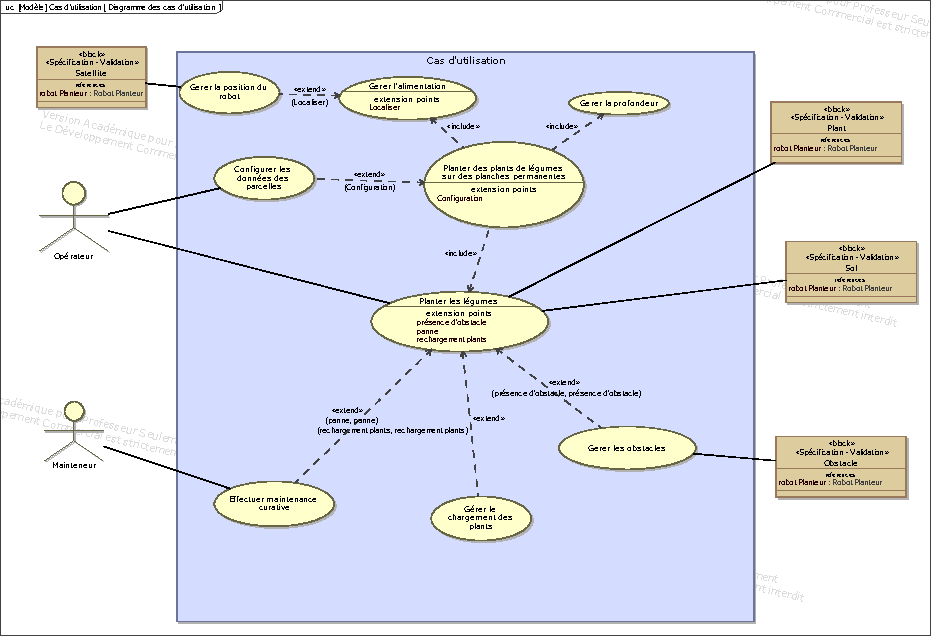
\includegraphics[width=.7\textwidth]{./I/images/casUtilisation.pdf}
\caption{Diagramme des cas d'utilisation}\label{fig:diagUC}
\end{figure} 
Nous avons placé dans l'ensemble de nos cas d'utilisation deux acteurs qui peuvent se dissocier : l'opérateur et le mainteneur. de manière assez naturelle, nous avons placé au centre des cas "Planter les légumes", point névralgique du système. De ce centre dépend plusieurs autres utilisations de notre système comme effectuer des maintenances, gestion des obstacles et des plants et enfin toute la partie de configuration du système.

\section{Scénarios et diagramme de séquence}
Nous avons fait le choix de ne traiter que 3 cas d'utilisation en scénarios et diagrammes de séquence.

\paragraph*{Cas d'utilisation 1 : Planter des choux}
Après que l’opérateur ait positionné le robot en position initiale, chargé 240 plants sur le robot et configuré la parcelle, il le met en marche.
Le robot avance, s’arrête sur la zone a planter puis charge un plant dans chaque buses. Les buses se positionnent sur la zone à planter, descendent, perforent le sol puis s'ouvrent pour laisser tomber les plants. Le cycle recommence jusqu’à arrivé en bout de planche ou le robot effectue une translation vers la droite pour se placer en bout de la planche suivante et répéter le cycle de plantation jusqu’à arrivé en bout de parcelle ou que le stock de plants soit vide.\begin{center}
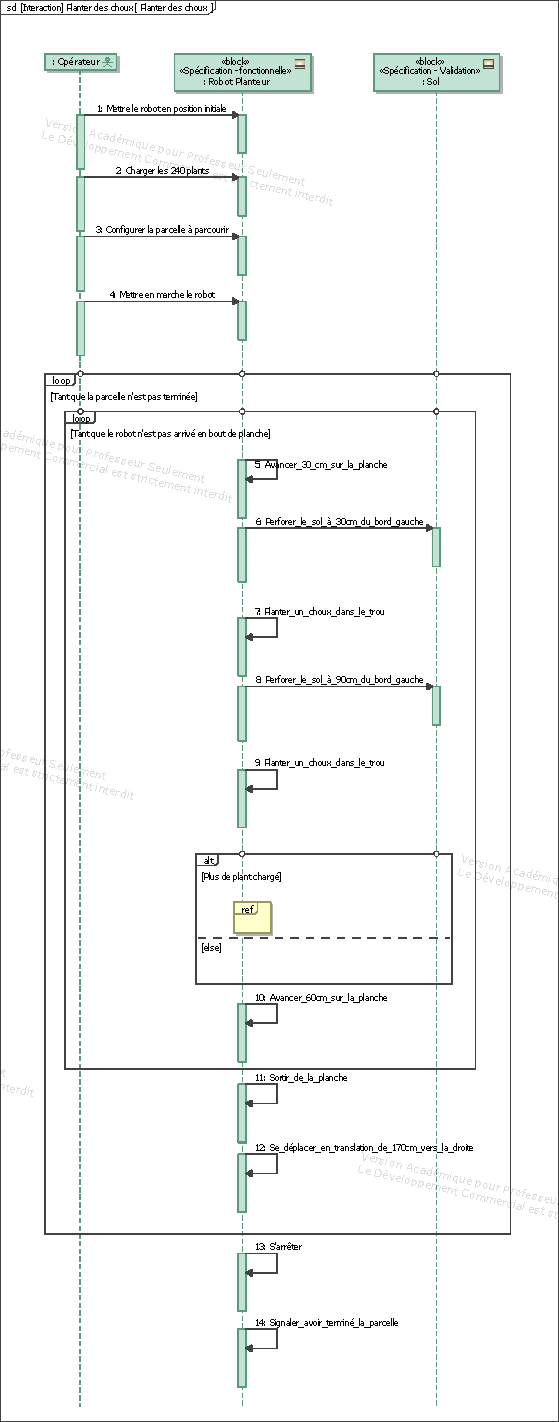
\includegraphics[width=.5\textwidth]{./I/images/planterChoux.pdf}
\captionof{figure}{Diagramme de séquence : Planter des choux}\label{fig:diagSeqPlanterChoux}
\end{center} 

\paragraph*{Cas d'utilisation 2: Gérer le chargement des plant}
Quand le robot détecte que son stock est vide, il enregistre son état actuel, il avertie ensuite l’opérateur à l'aide d'un signal physique puis se dirige en bout de planche. L’opérateur recharge le robot en plants, valide le chargement et le robot reprend la position sauvegarder précédemment et continue son cycle normal.%% Vraiment désolé, j'ai été obligé de passer cmme sa pour la faire tenir en place
\begin{center}
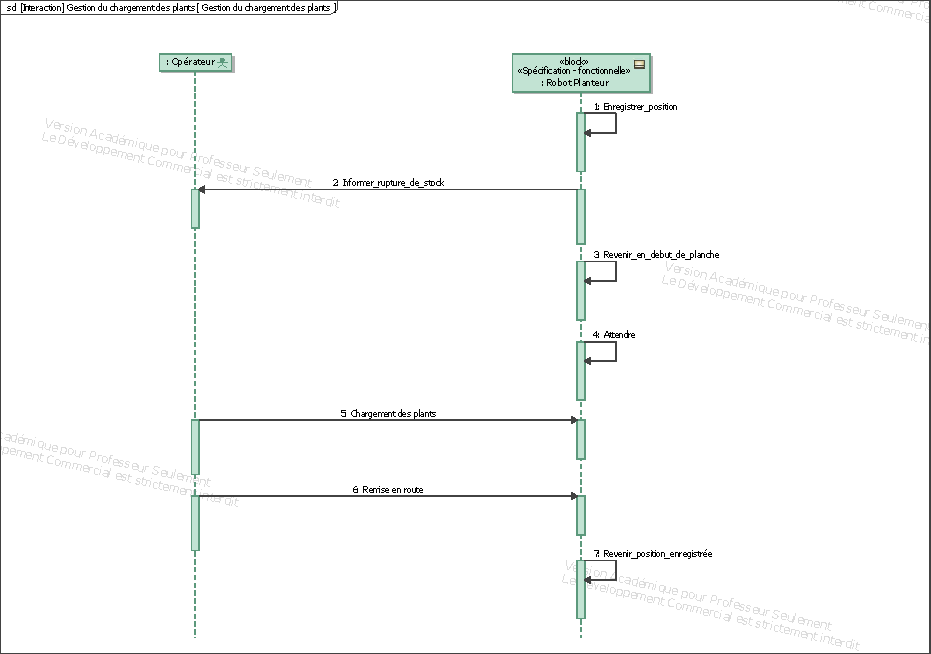
\includegraphics[width=.5\textwidth]{./I/images/gestionChargementPlant.pdf}
\captionof{figure}{Diagramme de séquence : Gestion du chargement des plants}\label{fig:diaggestionChargement}
\end{center} 


\paragraph*{Cas d'utilisation 3: Gérer les obstacles}
Lorsque un obstacle se présente devant le robot, il est détecté et le robot s'arrête. Il signale l'obstacle à l’opérateur à l'aide d'un signal physique. Pour que le robot reprenne son cycle normal l'obstacle ne doit plus être détecté par le robot et l’opérateur doit valider la remise en marche. 

\begin{figure}[!ht]
\centering
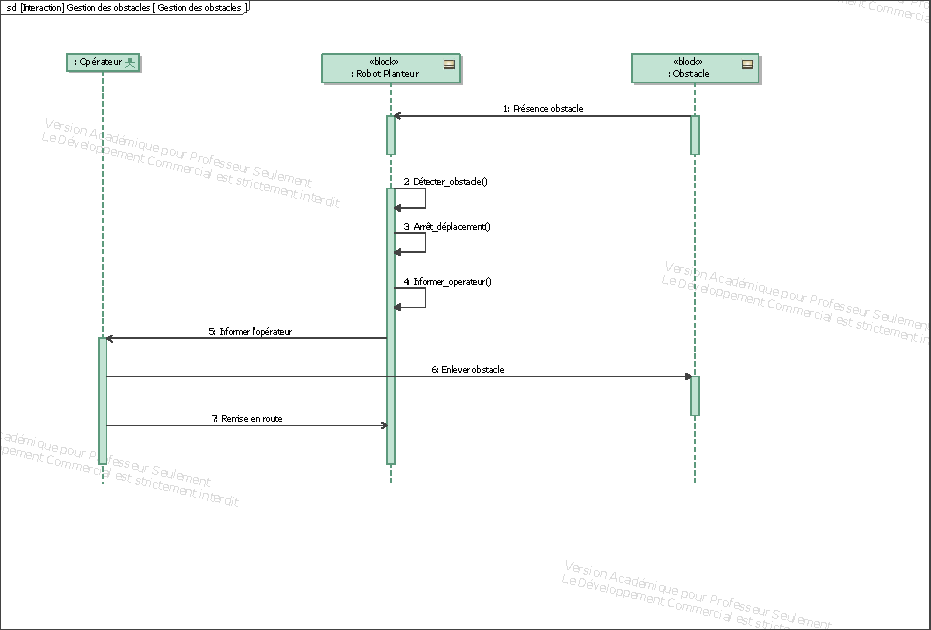
\includegraphics[width=.6\textwidth]{./I/images/gererObstacles.pdf}
\caption{Diagramme de séquence : Gérer les obstacles}\label{fig:diagSeqGereObstacle}
\end{figure}